

\author[Ben Deitmar]{Nix}


\logo{
\includegraphics[height=1cm]{Bilder/logo}}


\section{SDE$^M$VAE}

\begin{frame}
	\frametitle{Erste Verallgemeinerung: ODE M-ter Ordnung}
	Bisherige ODE:
	\begin{align*}
	\nabla s(\cdot,\omega) &= v(\cdot,\omega) \in \R^d\\
	\nabla v(\cdot,\omega) &= \bold{f}\big(s(\cdot,\omega),v(\cdot,\omega)\big) \in \R^d
	\end{align*}
	Verallgemeinerung für $M=3$:
	\begin{align*}
	\nabla s(\cdot,\omega) &= \bold{f}_1\big(s(\cdot,\omega),v(\cdot,\omega),w(\cdot,\omega)\big)\\
	\nabla v(\cdot,\omega) &= \bold{f}_2\big(s(\cdot,\omega),v(\cdot,\omega),w(\cdot,\omega)\big)\\
	\nabla w(\cdot,\omega) &= \bold{f}_3\big(s(\cdot,\omega),v(\cdot,\omega),w(\cdot,\omega)\big)
	\end{align*}
	Schreibe $\bm{\mu} = \bold{f} : \R^{M \times d} \rightarrow \R^{M \times d}$ und $z = (s,v,w)^T \in \R^{M \times d}$.
\end{frame}


\begin{frame}
	\frametitle{Zweite Verallgemeinerung: SDE}
	Bisherige ODE: \ \ $\forall k < M, \forall i \leq d :$
	\begin{align*}
	 & d z^{(k,i)}(t) = \bm{\mu}^{k,i}(z(t)) \, dt
	\end{align*}
	Verallgemeinerung für $\bm{\sigma} : \R^{M \times d} \rightarrow \R^{M \times d \times n}$:
	\begin{align*}
	& d z^{(k,i)}(t) = \bm{\mu}^{k,i}(z(t)) \, dt + \sum\limits_{j=1}^n \bm{\sigma}^{k,i,j}\big(z^{(0)}(t),...,z^{(M-1)}(t)\big) \, dW^j_t
	\end{align*}
	\rotatebox[origin=c]{180}{$\Lsh$} $(M \, d)$-dimensionale SDE mit Brownschen Bewegungen (BBs) $W^1,...,W^n$.
\end{frame}


\begin{frame}
	\frametitle{BB als Random Walk}
	\begin{itemize}
		\item Satz von Donsker:\\
		Seien $Y_1,Y_2,...$ uiv. mit $\E[Y_i]=0$ und $\sigma^2 := \E[Y_i^2] < \infty$.\\
		Definiere den Prozess
		\begin{align*}
		& W_{m,t} := \frac{1}{\sqrt{m}} \left( \sum\limits_{i=1}^{\lfloor mt \rfloor} Y_i + (mt - \lfloor mt \rfloor) Y_{\lfloor mt \rfloor +1}\right) \in C^0([0,\tau]) \ .
		\end{align*}
		Dann gilt $W_{m,\cdot} \xrightarrow{m \rightarrow \infty}_{\mathcal{L}} W$ (BB) in $C^0([0,\tau])$.
		
		\item Anschaulich:\\
		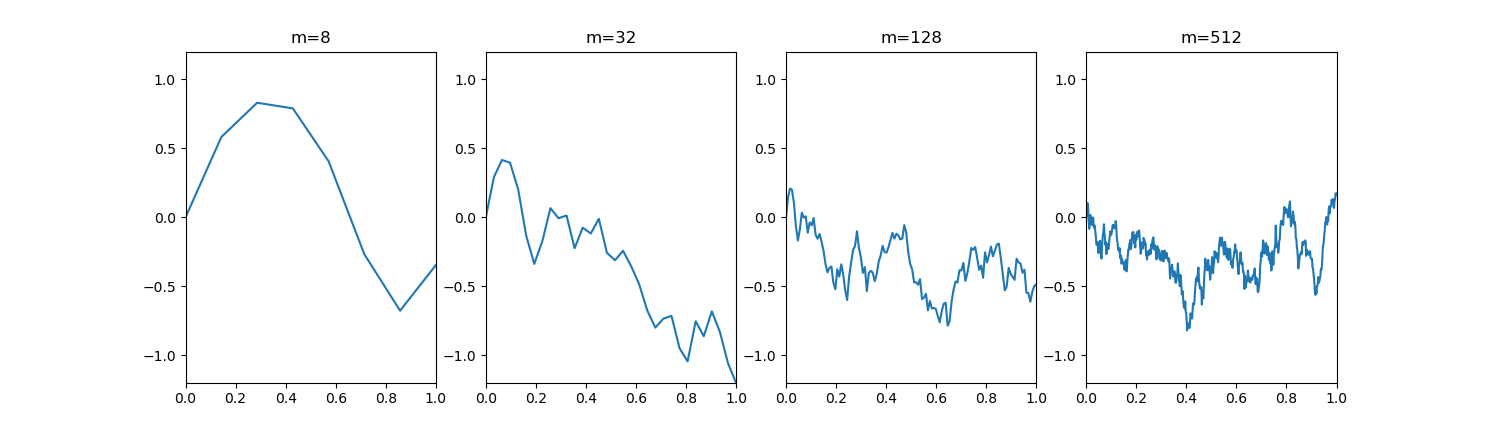
\includegraphics[scale=0.25]{Ben/DonskerBilder.png}
	\end{itemize}
	
\end{frame}


\begin{frame}
	\frametitle{SDE als ODE mit Random Walk}
	\begin{itemize}
		\item eindimensionale SDE:
		\begin{align*}
		& dX_t = \bm{\mu}(t,X_t) \, dt + \sum\limits_{j=1}^n \bm{\sigma}^{j}(t,X_t) \, dW^j
		\end{align*}
		\item Ito-Diffusion (nicht Zeit-abhängig):
		\begin{align*}
		& dX_t = \bm{\mu}(X_t) \, dt + \sum\limits_{j=1}^n \bm{\sigma}^{j}(X_t) \, dW^j
		\end{align*}
		\item Euler-Maruyama-Verfahren um Lösung $X$ zu approximieren:
		\begin{align*}
		& X_{m,t_k} := X_{m,t_{k-1}} + \Delta t^m \bm{\mu}(X_{m,t_{k-1}}) + \sqrt{\Delta t^m} \sum\limits_{j=1}^n \bm{\sigma^j}(X_{m,t_{k-1}}) \underbrace{\varepsilon_{j,k}}_{\sim \mathcal{N}(0,1)}
		\end{align*}
		Für $0=t_0<...<t_m=\tau$ mit $t_k = k \frac{\tau}{m}$ und $\Delta t^m = \frac{\tau}{m}$.
	\end{itemize}
	
\end{frame}


\begin{frame}
	\frametitle{Lernen von $\bm{\mu}(0)$ und $\bm{\sigma}(0)$}
	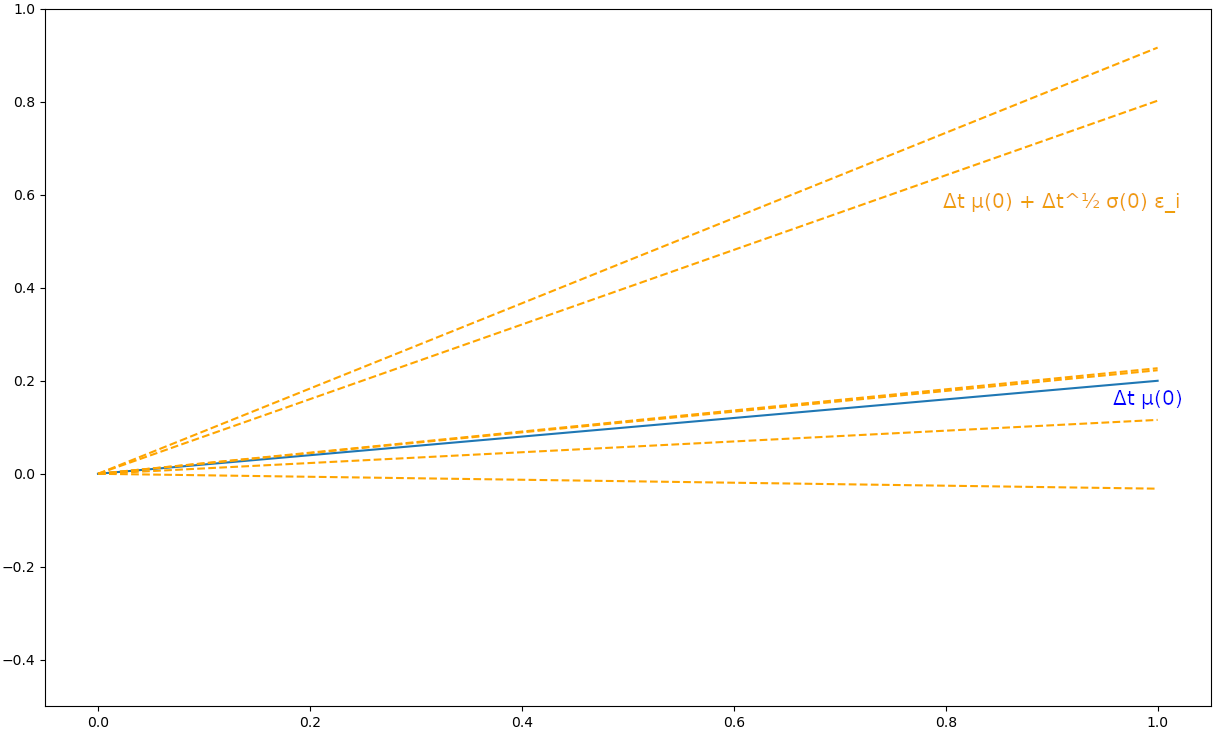
\includegraphics[scale=0.3]{Bilder/SDE_Erklaerung.png}
	
\end{frame}


\begin{frame}
	\frametitle{SDE-VAE Modell für $M=1$}
	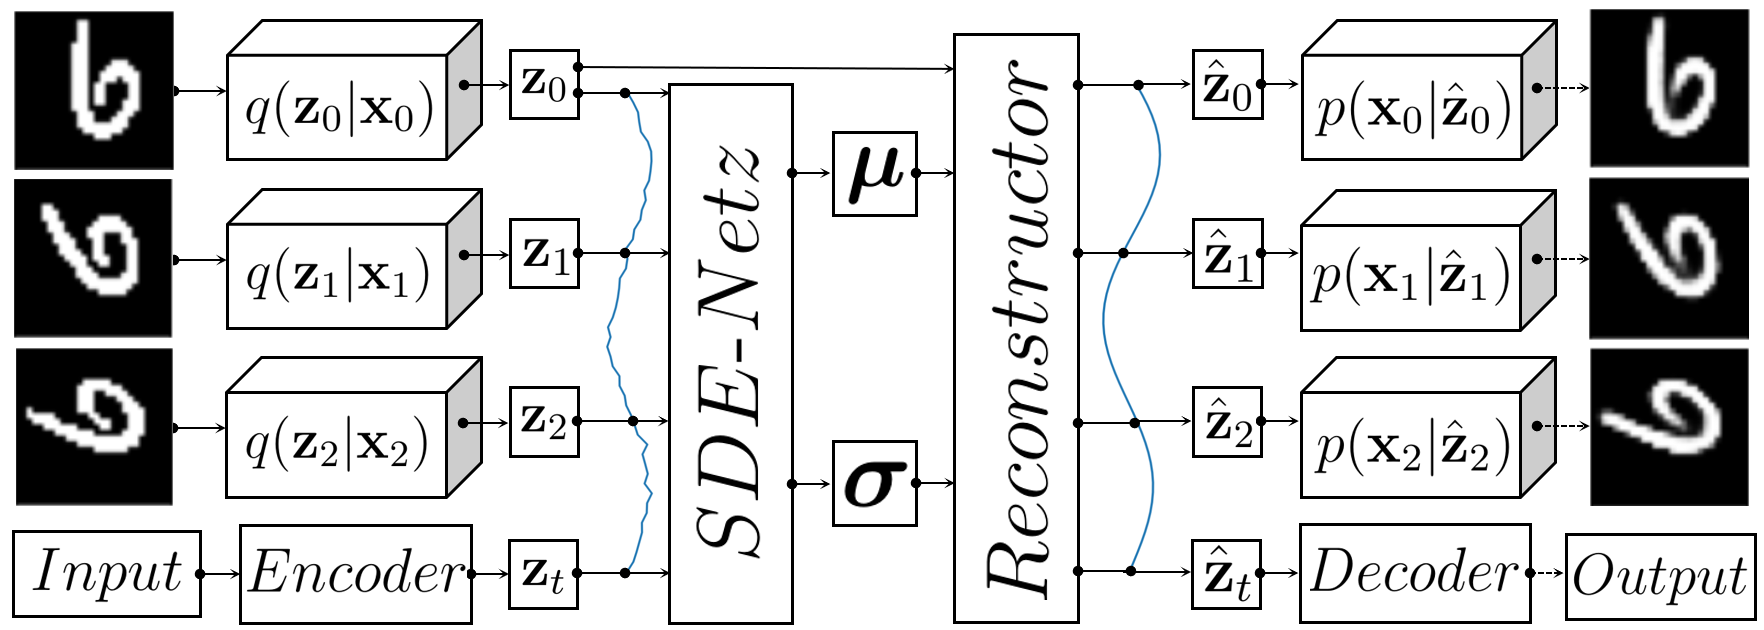
\includegraphics[scale=0.3]{Bilder/SDEVAEGrafik.png}
\end{frame}


\begin{frame}
	\frametitle{SDE-Ball-Datensatz}
	\begin{itemize}
		\item SDE:
		\begin{align*}
		& dX^1_t = X^2_t \, dt + 0,2 \, dW^1_t\\
		& dX^2_t = -X^1_t \, dt + 0,1 \, dW^1_t\\
		& X_0 = (0,1)
		\end{align*}
		
		\item Datensatz:\\
		Bilder von einem Ball, dessen Höhe durch $X^1_t$ gegeben ist.\\
		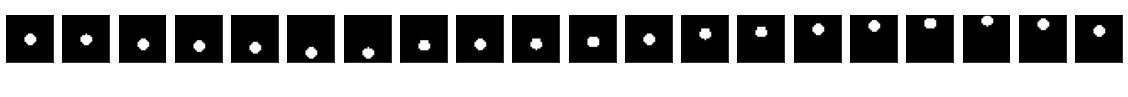
\includegraphics[scale=0.25]{Bilder/datasetSDE.png}
	\end{itemize}
\end{frame}

\begin{frame}
	\frametitle{Ergebnisse (SDE-Ball)}
	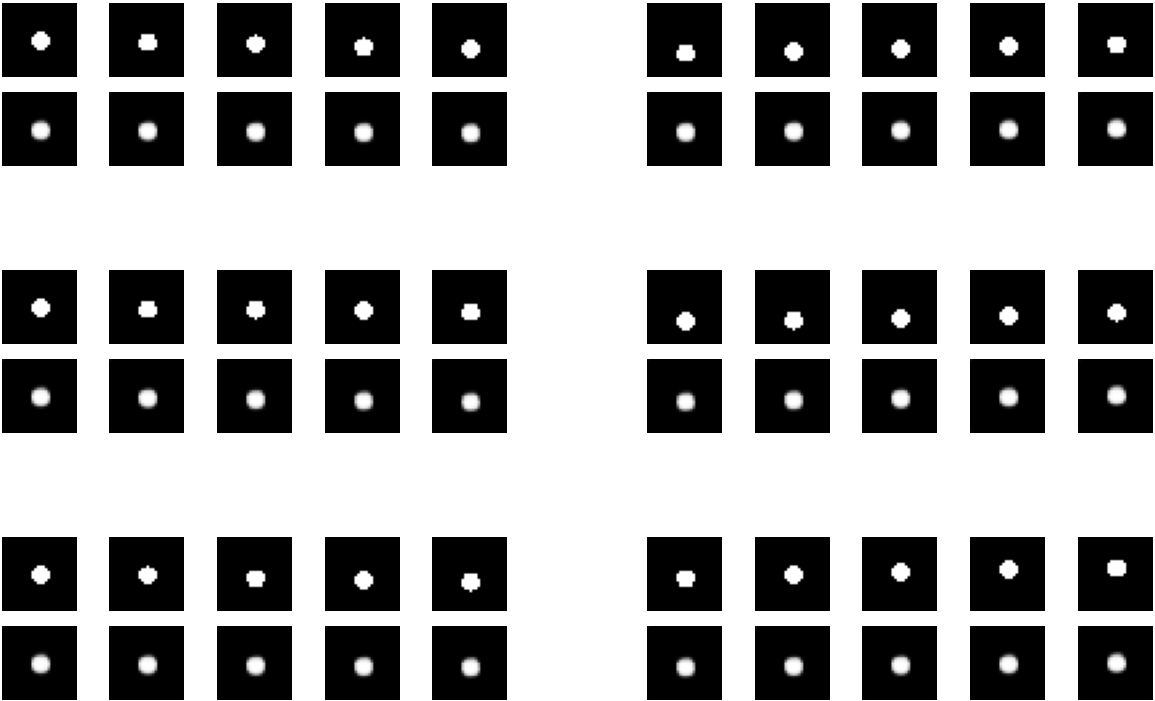
\includegraphics[scale=0.3]{Bilder/SDE_Ball_rec.png}
\end{frame}

\begin{frame}
	\frametitle{Ergebnisse (SDE-Ball)}
	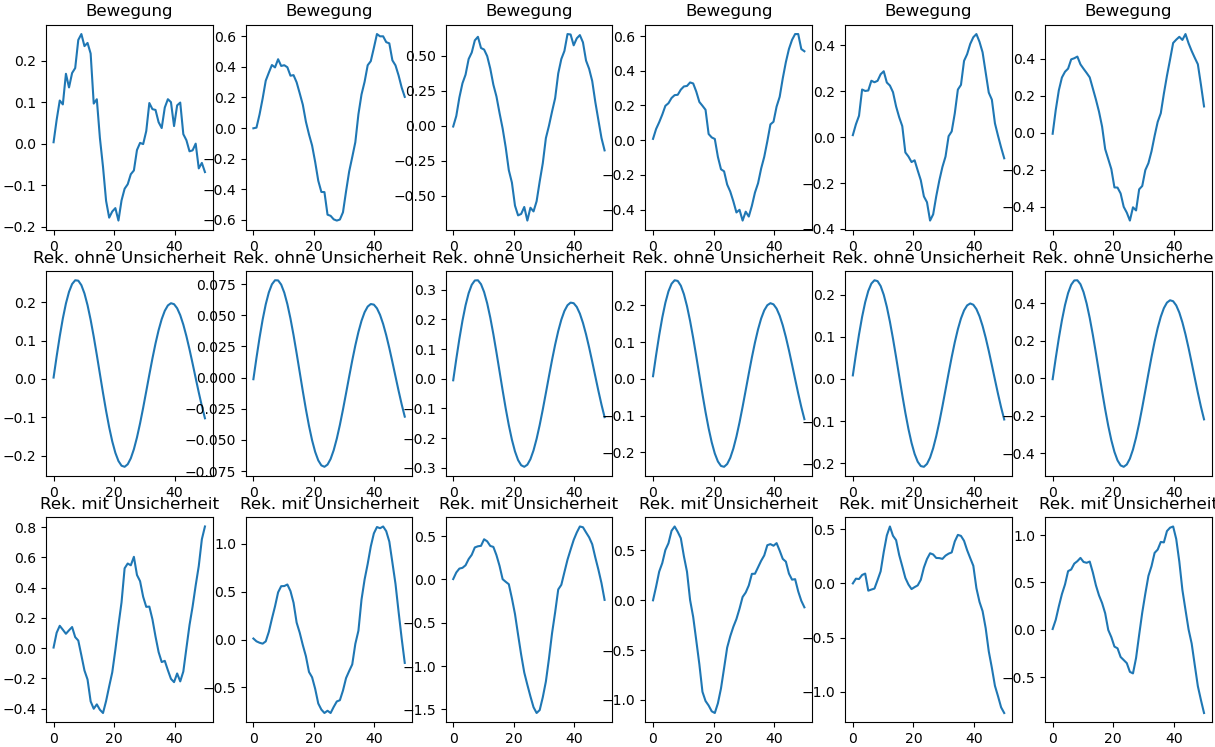
\includegraphics[scale=0.3]{Bilder/SDE_Ball_Ergebnisse.png}
\end{frame}


\begin{frame}
	\frametitle{Ergebnisse (rotMNIST)}
	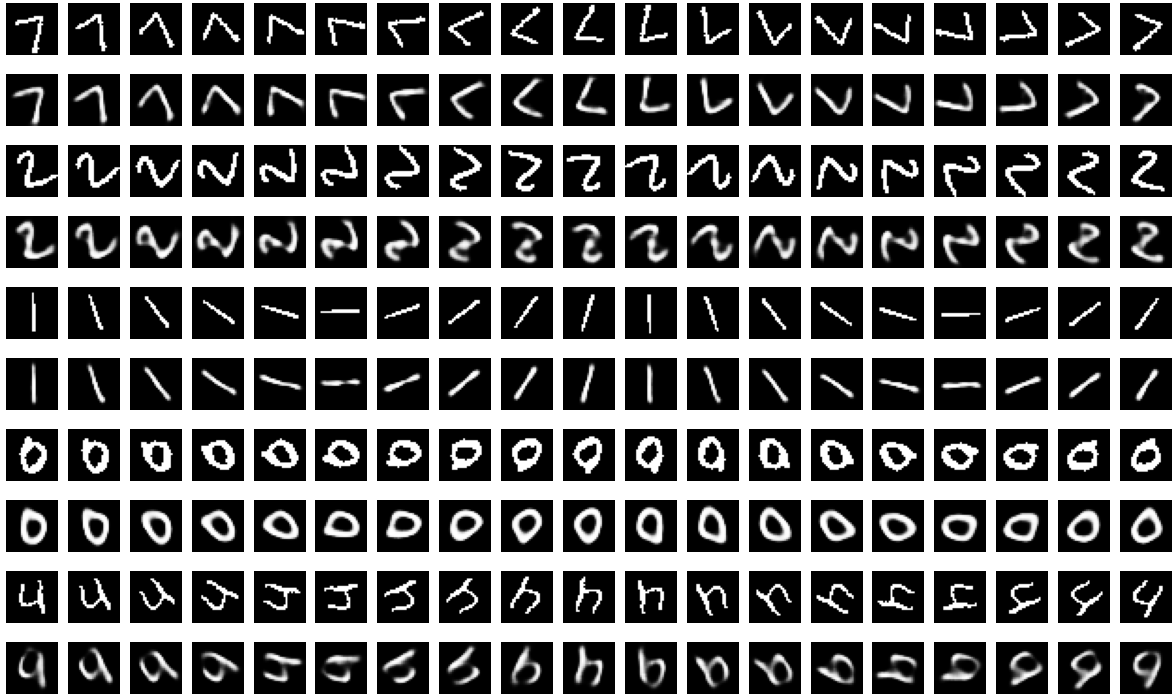
\includegraphics[scale=0.3]{Bilder/SDE_rotMNIST_rec}
\end{frame}

\begin{frame}
	\frametitle{Ergebnisse (rotMNIST)}
	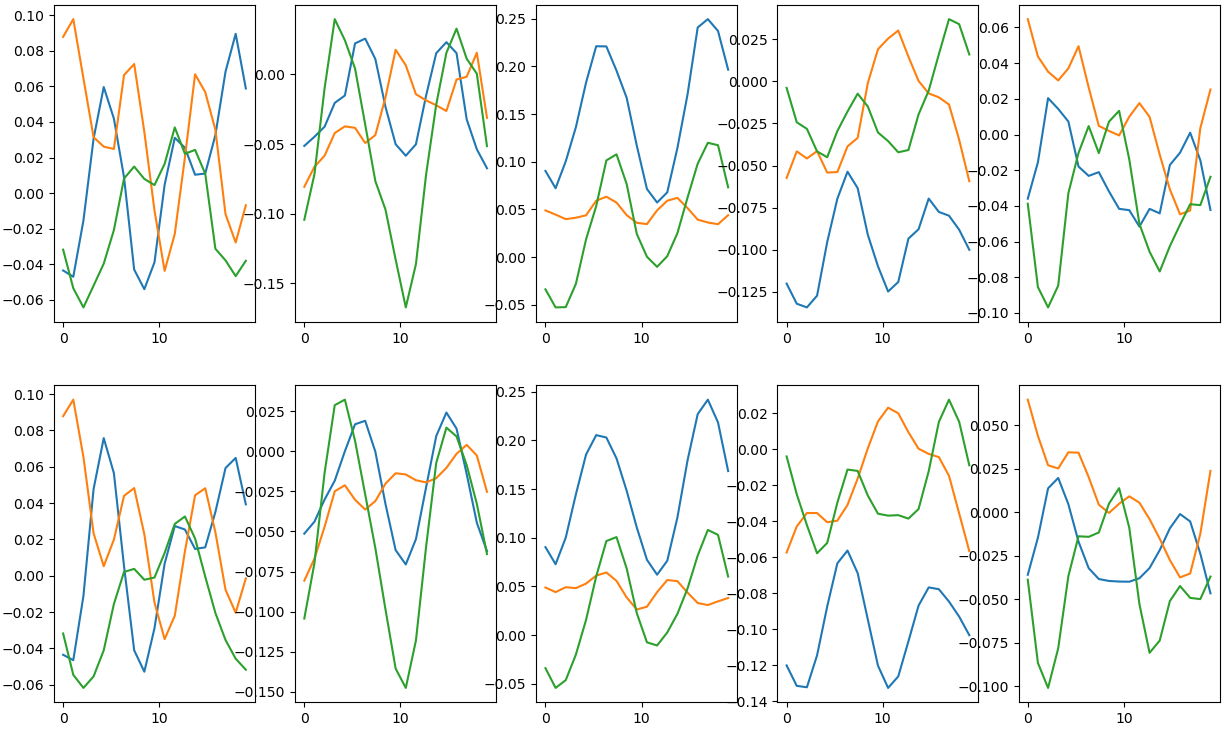
\includegraphics[scale=0.3]{Bilder/SDE_rotMNIST_latent_three_rec}
\end{frame}














